\subsection{设参}
在学习一次函数时,我们就接触过设参,设参思想是处理二次函数综合问题的核心代数化策略,其本质是通过引入辅助变量(称为参数)将几何动态问题转化为可计算的代数模型。当抛物线上的点$P$位置变化时,设其横坐标为参数$t$,根据二次函数解析式 $y = ax^2 + bx + c$,点$P$的纵坐标可直接用含$t$的代数式表示为:
\[
y = at^2 + bt + c
\]
此时点$P$的完整坐标可记为:
\[
P(t,\  at^2 + bt + c)
\].该操作的数学意义在于:
\begin{enumerate}
    \item 将连续运动的点转化为连续变化的参数.
    \item 通过特定条件控制参数的取值,用于描述几何关系
\end{enumerate}
\begin{remark}
设参的前提是明确所求的目标,不要为了设参而设参    
\end{remark}


\begin{example}
如图\ref{fig:sp1},抛物线 \( y = -x^2 + 2x + 3 \) 与 \( x \) 轴交于 \( A \),\( B \) 两点,与 \( y \) 轴交于 \( C \) 点。
\begin{enumerate}
    \item 直接写出 \( A, B, C \) 点的坐标;  
    \item 过点 \( A \) 作两条直线分别交抛物线于第一象限点 \( P, Q \),交 \( y \) 轴于点 \( M, N, OM \cdot ON = n \)。当 \( n \) 为定值时,直线 \( PQ \) 是否必定经过某一定点?若经过,请你求出该定点坐标(用含 \( n \) 的式子表示);若不经过,请说明理由。
\end{enumerate}
\end{example}

\begin{wrapfigure}{r}{4cm}
    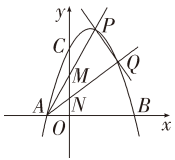
\includegraphics[width=1\linewidth]{figure/设参题1.png}
    \caption{}
    \label{fig:sp1}
\end{wrapfigure}

\begin{solution}
    分析:第一题:题目要求直接写出三个点的坐标,观察图像可以发现\(A,B\)两点是与\(x\)轴的交点,\(C\)点是与\(y\)轴的交点,题目给出了抛物线的一般式,能直接得出\(C\)点坐标为\((0,3\),观察解析式发现可以因式分解(十字相乘)将解析式写成交点式,即可得出\(A,B\)坐标为\(A(-1,0),B(3,0)\).
    
    第二题:题目实际上要求出直线\(PQ\)经过的定点,但是题目明显没有给出直线的解析式,此时就需要我们设出\(PQ\)的解析式为\(PQ:y=kx+m\) ,要求\(PQ\)先求\(P,Q\)两点,因为\(P,Q\)两点在抛物线上,也就是\(PQ\)与抛物线的两个交点,所以联立直线和抛物线得到\(kx+m=-x^2+2x+3\)整理可得\(x^2+(k-2)x+(m-3)\),由于过定点所以必定要消去\(m\)或者用代数式表示\(m\),因为题目要求用含\(n\)的代数式表达定点,所以\(m\)必定是一个含\(n\)的代数式,接下来尝试求\(m\),题目中给出的关于\(n\)的信息只有\(OM \cdot ON = n \),观察图像发现\(OM,ON\)实际上表示的是\(|y_M|\)和\(|y_N|\) 实际上是\(M,N\)两点的纵坐标,而这两点又是在两条直线\(PA,QA\)上,要想求\(M,N\)两点就得求直线\(PA,QA\),由上一题已知\(A(-1,0)\),还差\(P,Q\)的坐标才能分别求出两条直线\(PA,QA\)的解析式,而\(P,Q\)恰好在抛物线上,是抛物线与直线\(PQ\)的交点,就此我们建立了两个不同条件的关系(前面联立的方程就是抛物线与直线\(PQ\)的交点的方程),那么整理过的\(x^2+(k-2)x+(m-3)\)如何表达两个交点呢,显然可以运用韦达定理,两根之和等于二次项系数,两根之积等于常数项.
    
    此时设\(P(a,-a^2+2a+3),Q(b,-b^2+2b+3)\),根据韦达定理两根之和等于二次项系数,两根之积等于常数项,所以\(a+b=k-2, ab=m-3\),像要求\(M,N\)就需要求\(PA,QA\),现在已经设出\(P,Q\),因为两点确定一条直线,所以可以求出\(PA,QA\)的解析式分别为\(y=(3-a)(x+1),y=(3-a)(x+1)\),接下来就能求\(M,N\),因为\(M,N\)的横坐标都是0,所以代入求得\(M(0,a-3),N(0,b-3)\),所以\(OM=a-3,ON=b-3\),代入\( M, N, OM \cdot ON = n \),得\((a-3)(b-3)=n\),整理得\(ab-3(a+b)+9-n=0\),将\(a+b=k-2, ab=m-3\)代入该式得\(m=n-3k\),这样就达成了我们最初的目的,最后将\(m=n-3k\)代入\(PQ:y=kx+m\)就能得到\(PQ\)过定点$(3,n)$,注意写解前要先说:\(PQ\)过定点,再写过程.
\end{solution}